% Autor: Leonhard Segger, Alexander Neuwirth
% Datum: 2017-10-30
\documentclass[
	% Papierformat
	a4paper,
	% Schriftgröße (beliebige Größen mit „fontsize=Xpt“)
	12pt,
	% Schreibt die Papiergröße korrekt ins Ausgabedokument
	pagesize,
	% Sprache für z.B. Babel
	ngerman
]{scrartcl}

% Achtung: Die Reihenfolge der Pakete kann (leider) wichtig sein!
% Insbesondere sollten (so wie hier) babel, fontenc und inputenc (in dieser
% Reihenfolge) als Erstes und hyperref und cleveref (Reihenfolge auch hier
% beachten) als Letztes geladen werden!

% Silbentrennung etc.; Sprache wird durch Option bei \documentclass festgelegt
\usepackage{babel}
% Verwendung der Zeichentabelle T1 (Sonderzeichen etc.)
\usepackage[T1]{fontenc}
% Legt die Zeichenkodierung der Eingabedatei fest, z.B. UTF-8
\usepackage[utf8]{inputenc}
% Schriftart
\usepackage{lmodern}
% Zusätzliche Sonderzeichen
\usepackage{textcomp}

% Mathepaket (intlimits: Grenzen über/unter Integralzeichen)
\usepackage[intlimits]{amsmath}
% Ermöglicht die Nutzung von \SI{Zahl}{Einheit} u.a.
\usepackage{siunitx}
% Zum flexiblen Einbinden von Grafiken (\includegraphics)
\usepackage{graphicx}
% Abbildungen im Fließtext
\usepackage{wrapfig}
% Abbildungen nebeneinander (subfigure, subtable)
\usepackage{subcaption}
% Funktionen für Anführungszeichen
\usepackage{csquotes} 
\MakeOuterQuote{"}
% Zitieren, Bibliographie
\usepackage{biblatex}


% Zur Darstellung von Webadressen
\usepackage{url}
%chemische Formeln
\usepackage[version=4]{mhchem}
% siunitx: Deutsche Ausgabe, Messfehler getrennt mit ± ausgeben
\usepackage{floatrow}
\floatsetup[table]{capposition=top}
\usepackage{float}
% Verlinkt Textstellen im PDF-Dokument
\usepackage[unicode]{hyperref}
% "Schlaue" Referenzen (nach hyperref laden!)
\usepackage{cleveref}
\sisetup{
	locale=DE,
	separate-uncertainty
}
%\bibliography{6Mi_M3_29-11-2017_References}
%TODO anpassen

\begin{document}
	
	\begin{titlepage}
		\centering
		{\scshape\LARGE Versuchsbericht zu \par}
		\vspace{1cm}
		{\scshape\huge W1 - Stirling-Motor \par} 
		\vspace{2.5cm}
		{\LARGE Gruppe 14Mo \par}
		\vspace{0.5cm}
		
		{\large Alexander Neuwirth (E-Mail: a\_neuw01@wwu.de) \par}
		{\large Leonhard Segger (E-Mail: l\_segg03@uni-muenster.de) \par}
		\vfill
		
		durchgeführt am 14.05.2018\par 
		betreut von\par
		{\large Torsten Stiehm} 
		
		\vfill
		
		{\large \today\par}
	\end{titlepage}
	\tableofcontents
	\newpage

	\section{Kurzfassung}
	%TODO Hypothese	und deren Ergebnis, wenn Hypothese ist, dass nur Theorie erfüllt, sagen: Erwartung: Theorie aus einführung (mit reflink) erfüllt
	%TODO Ergebnisse, auch Zahlen, mindestens wenn's halbwegs Sinn ergibt
	%TODO Was wurde gemacht
	%TODO manche leute wollen Passiv oder "man", manche nicht
	
	\section{Methoden} \label{sec_Methoden}
	%TODO Bilder von der Website klauen
	
	%TODO Motor frequenz FFT
	%TODO 5 fach millilitter für Durchfluss
	
	\section{Ergebnisse und Diskussion}
	%TODO Unsicherheiten
	

	\subsection{Beobachtung}
	%TODO Einflüsse von veränderten Parametern auf Messung
	
	%TODO Schmilz Wasser bla
	\subsection{Datenanalyse}
	
	\subsubsection{Unsicherheiten} 
	Die Unsicherheiten wurden gemäß GUM ermittelt. 
	Außerdem wurde für Unsicherheitsrechnungen die Python Bibliothek "uncertainties" verwendet.
	\begin{description}
		\item[Messzylinder] Die Unsicherheit des Messzylinders wurde mit \SI{0,04}{mL} abgeschätzt (dreieckige WDF).
		\item[Stoppuhr] Die Stoppuhr zeigt Sekunden mit Zwei Nachkommastellen an, woraus eine Unsicherheit von \SI{0,004}{s} folgt (rechteckige WDF), jedoch hat die Reaktionszeit einen größeren Einfluss, wesshalb eine Unsicherheit von \SI{0,1}{s} angenommen wird. 
		\item[Pipette] Auf der Pipette, die zum Füllen des Reagenzglases m Zylinderkopf verwendet wurde, ist eine Unscherheit von \SI{0,007}{mL} angegeben.
		\item[Thermometer] Die Unsicherheit des Kühlwasserthermometers vom Typ K ist \SI{1,5}{\degreeCelsius} in dem gemessenen Temperaturinterval. Da diese für das Messen von Temperaturdifferenzen kaum Einfluss hat, werden die Unsichereiten aufgrund der Schwankungen mit \SI{0,05}{\degreeCelsius} abgeschätzt.
		\item[Motorfrequenz] Die Unsicherheit der, durch FFT ermittelten, Frequenzen wurde mit \SI{0,01}{Hz} abgeschätzt, da die Frequenz kaum schwankte und keine anderen Frequenzen im FFT auftraten.
	
	\end{description}
	\subsubsection{Bestimmung der Reibungsverluste}
	Die Reibungsverluste lassen sich aus der Erwärmung des Kühlwassers beim Betrieb der Wärmepumpe bzw. Kältemaschine bei offenem Zylinderkopf bestimmen.
	Die zugeführte Wärmemenge $\Delta{Q}$ ist proportional zur Temperaturänderung $\Delta{T}$:
	\begin{equation}
	\Delta{Q} = C_W \cdot \Delta{T} = c \cdot m \cdot \Delta{T}
	\label{eq_Wärme}
	\end{equation} 
	Für Wasser beträgt die spezifische Wärme $c_{H_2O}$ = \SI{4,185}{J/g/K}.
	Die Masse $m$ im System ist nicht direkt bestimmbar, der Durchfluss des Kühlwasser $d=m/t$ hingegen schon. %TODO Besserer Satz?
	Somit lässt sich mit \cref{eq_Wärme} die an das Kühlwasser abgegebenen Leistung $\Delta{Q}/t$ ermitteln.
	Die gesuchte Reibungsarbeit pro Umlauf erhält man durch Division der Leistung durch die Frequenz des Motors.
	Es folgt:
	\begin{equation}
	W_R = c_{H_2O} \cdot \frac{d}{f} \cdot \Delta{T}
	\label{eq_Reibungsarbeit}
	\end{equation}
	Der Durchfluss d ergibt sich indem man die geflossene Wassermenge $v$ durch die gestoppte Zeit $t$ dividiert und mit der Dichte $\rho_{H_2O}$ multipliziert. Aus \cref{tab_Durchfluss} ergibt sich ein Mittelwert von \SI{4,61+-0,13}{mL/s} und somit ein Durchfluss d = \SI{4,61+-0,13}{g/s}.
	
	Die Frequenz des Motors wurde mittels FFT auf \SI{3,15+-0,01}{Hz} eingestellt (vgl. \cref{sec_Methoden}).
	Die Temperaturänderung des Kühlwassers $\Delta{T}$ betrug \SI{0,5+-0,05}{\degreeCelsius}.
	Es folgt eine Reibungsarbeit pro Umlauf gemäß \cref{eq_Reibungsarbeit} von $W_R=\SI{2,76+-0,29}{J}$.
	\begin{table}[H]
		\centering
		\begin{tabular}{ c | c }
			Wassermenge $v$ in \SI{}{mL} & Zeit $t$ in \SI{}{s} \\ \hline
			\SI{38,0+-0,03}{}&\SI{8,16+-0,1}{}\\
			\SI{40,8+-0,03}{}&\SI{8,50+-0,1}{}\\
			\SI{41,4+-0,03}{}&\SI{9,34+-0,1}{}\\
			\SI{49,2+-0,03}{}&\SI{10,78+-0,1}{}\\
			\SI{47,0+-0,03}{}&\SI{10,22+-0,1}{}\\
		\end{tabular}
		\caption{Gemessene Kühlwassermenge die durch den Striling-Motor in einer bestimmten Zeit fließt.}
		\label{tab_Durchfluss} 
	\end{table}
	
	\subsubsection{Bestimmung der Kühlleistung} \label{sssec_Kühlleistung}
	Die pro Umlauf aufzuwendende mechanische Arbeit $-W$ ist durch
	\begin{equation}
	W =  Q_1 - Q_2 + W_R
	\end{equation}
	gegeben.
	Die Wärme $Q_2$ wird dem Zylinderkopf pro Umlauf entzogen und die Wärme $-Q_1$ wird dem Kühlwasser zu geführt.
	
	$Q_1+W_R$ lässt sich analog zur Reibungsarbeit pro Umlauf mit \cref{eq_Reibungsarbeit} bestimmen.	
	Die gemessene Temperaturänderung des Kühlwassers betrug $\Delta{T}$=$\SI{1,0+-0,05}{\degreeCelsius}$ woraus $Q_1+W_R$=$\SI{5,53+-0,33}{J}$ folgt.
	
	$Q_2$ ergibt sich aus der Steigung der Messkurve in \cref{fig_Kuehl}.
	Es wurde ein linearer Fit verwendet, um die Steigung nahe der Raumtemperatur zu Bestimmen.
	Die Kühlleistung $P_\text{Kühl}$ ist gegeben durch zeitliches Ableiten von \cref{eq_Wärme}.
	\begin{equation}
	\dot{Q} = P_\text{Kühl} = c \cdot m \cdot s = c \cdot \rho \cdot V \cdot s
	\label{eq_Kühlleistung}
	\end{equation}
	
	Mittels Division der Kühlleistung $P_\text{Kühl}$ durch die Frequenz des Motors erhält man die Wärme $Q_2$ pro Umlauf:
	\begin{equation}
	Q_2 = \frac{P_\text{Kühl}}{f} = c \cdot \rho \cdot V \cdot \frac{s}{f}	
	\end{equation}
	In dem Reagenzglas im Zylinderkopf befand sich $V$=\SI{1+- 0,007}{mL} destilliertes Wasser und die Steigung $s$ beträgt $\SI{0,2002+-0,0002}{\degreeCelsius/s}$. %TODO Satz
	Folglich ist $P_\text{Kühl}$ = \SI{0,838+-0,006}{W} und $Q_2$ = $\SI{0,266+-0,002}{J}$.
	
	Die Leistungszahl $\epsilon$ ist der Quotient der entnommenen Wärmemenge $Q_2$ und aufgewandter Arbeit $W$:
	\begin{equation}
		\epsilon = \frac{|Q_2|}{|W|}
		\label{eq_Leistungszahl}
	\end{equation}
	Hier beträgt $W=Q_1+W_R-Q_2=\SI{5,26+-0,33}{J}$ woraus eine Lesitungszahl von $\epsilon$ = $\SI{5,1 +- 0,3}{\%}$ folgt.
	
	\begin{figure}[H]
		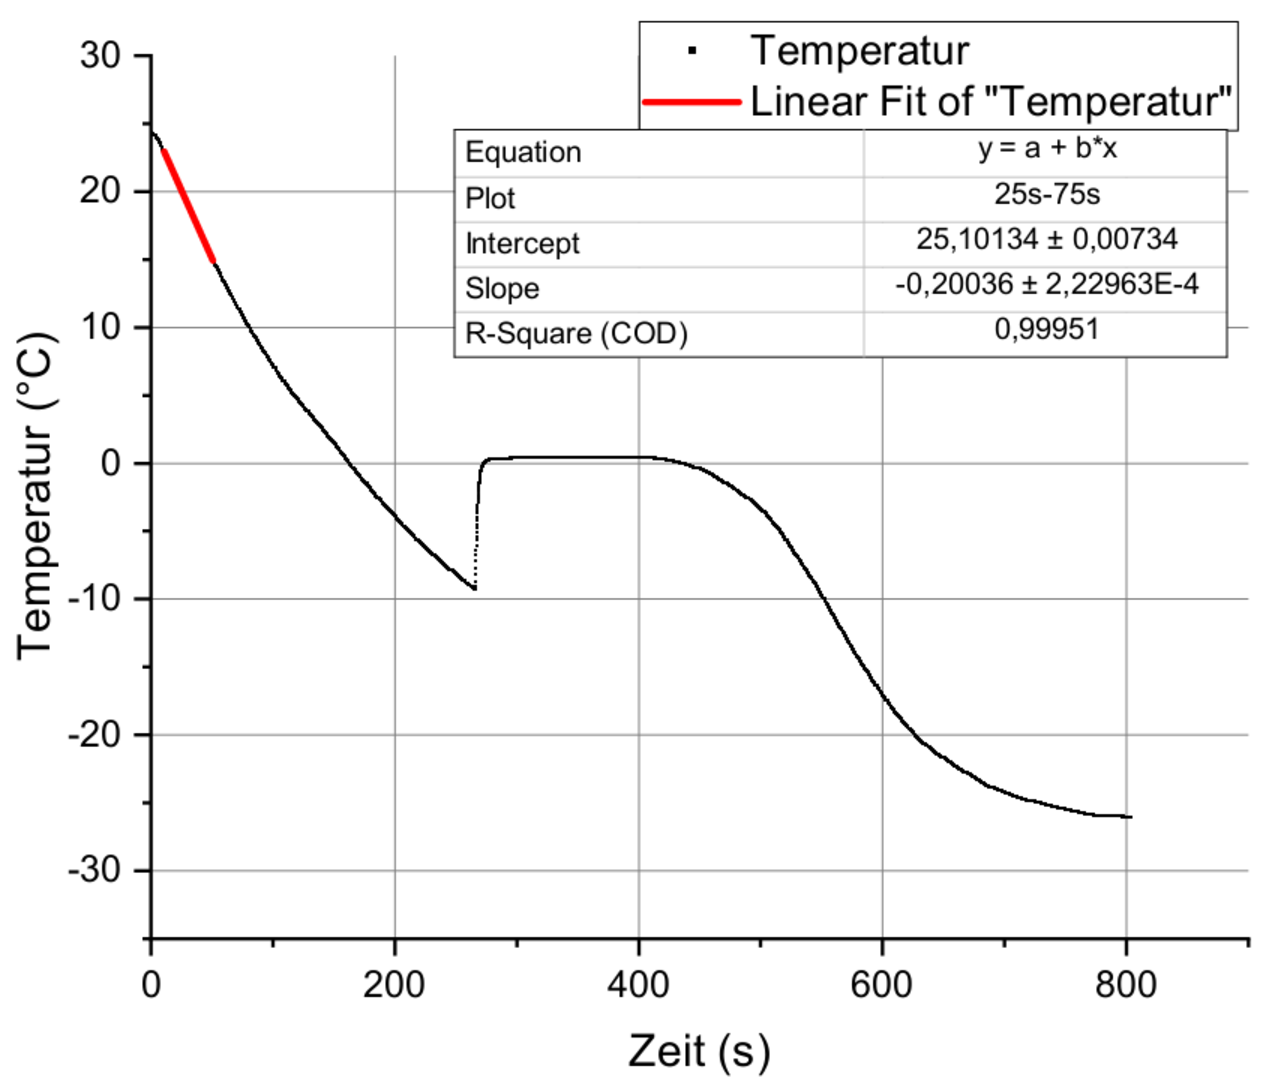
\includegraphics[width=0.7\textwidth]{Kuehl}
		\centering
		\caption{Gemessene Temperatur als Funktion der Zeit beim betreiben des Striling-Motors als Kältemaschine. Die Fehler sind kleiner als die Symbole.}
		\label{fig_Kuehl}
		\centering
	\end{figure}

	Unter der Annahme, dass der Motor der Probe konstant Wärme entzieht, lässt sich die von dem Wasser beim Schmelzen abgegebene Wärme anhand von \cref{fig_Kuehl} abschätzen.
	Im Zeitraum von \SI{266+-2}{s} bis \SI{545+-5}{s} entzieht der Motor dem Wasser Wärme, die Anfangs- und Endtemperatur sind jedoch gleich. 
	Folglich entspricht die entzogene Wärme pro Masse der Schmelzwärme $S$ = \SI{233,7+-4.5}{J/g}, gemäß:
	\begin{equation}
	S = \frac{Q}{m} = c \cdot s\cdot \Delta{t}
	\end{equation}
	
	
	
	\subsubsection{Bestimmung der Heizleistung}
	Die Heizleistung lässt sich analog zur Kühlleistung in \cref{sssec_Kühlleistung} aus der Steigung $s_\text{l}$ der Messkurve bei Raumtemperatur in \cref{fig_Waerm} bestimmen.
	
	Die Steigung $s_\text{l}$ beträgt \SI{0,377+-0,001}{\degreeCelsius/s} somit folgt aus \cref{eq_Kühlleistung} eine Heizleistung $P_\text{Heiz}$ von \SI{1,58+-0,01}{W}.
	%TODO CHECK START
	Analog lässt sich auch die Leistungszahl $\epsilon$ bestimmen. 
	Die Temperaturänderung $\Delta{T}$ betrug $\SI{0,3+-0,05}{\degreeCelsius}$ woraus gemäß \cref{eq_Reibungsarbeit} ein $Q_1+W_R$ von $\SI{1,66+-0,28}{J}$ folgt. 
	$Q_2$ ergibts sich aus $P_\text{Heiz}/f$=\SI{0,501+-0,004}{J}. %TODO CREFS auf gleichungen
	Die Leistungszahl beträgt somit \SI{43,1+-10,4}{\%}.
	\begin{figure}[H]
		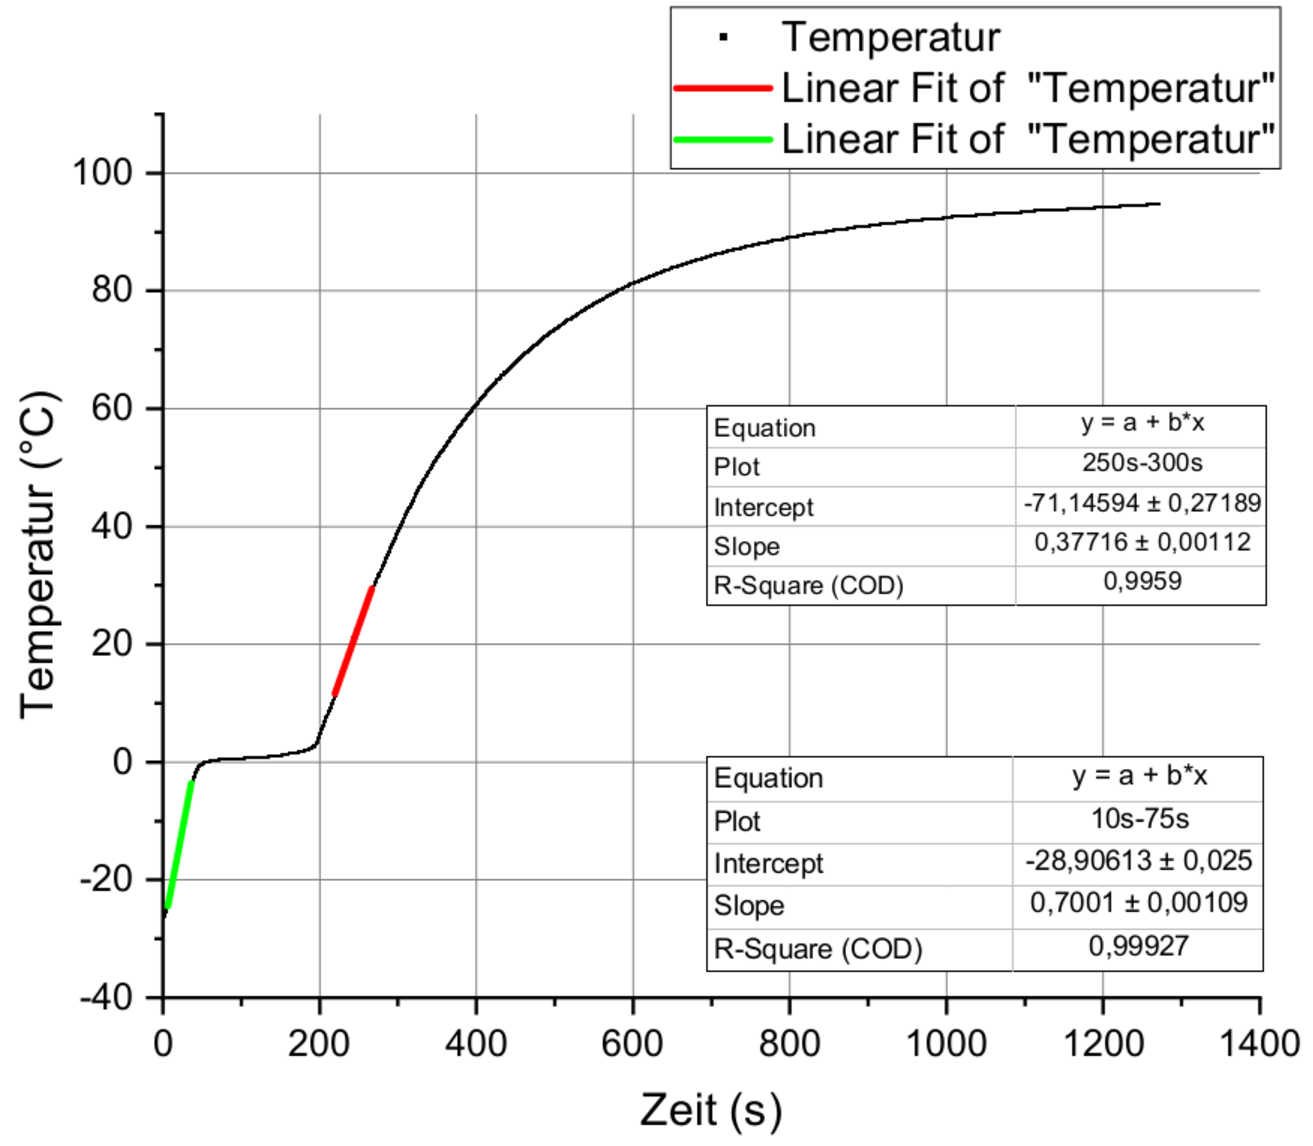
\includegraphics[width=0.7\textwidth]{Waerm}
		\centering
		\caption{Gemessene Temperatur als Funktion der Zeit beim betreiben des Striling-Motors als Wärmepumpe. Die Fehler sind kleiner als die Symbole.}
		\label{fig_Waerm}
		\centering
	\end{figure}
	%TODO CEHCK END
	Die spezifische Wärme von Eis lässt sich aus \cref{eq_Kühlleistung} bestimmen:
	\begin{equation}
		c_\text{Eis} = \frac{P_\text{Heiz}}{m \cdot s_\text{s}} = c_{H_2O} \frac{s_\text{l}}{s_\text{s}}
	\end{equation} 
	Die Steigung $s_\text{s}$ nimmt einen Wert von \SI{0,700+-0,001}{\degreeCelsius/s} im Bereich von \SI{-25}{\degreeCelsius} bis \SI{-5}{\degreeCelsius} an. 
	Es ergibt sich eine spezfische Wärme für Eis $c_\text{Eis}$ von $\SI{2,254+-0,007}{J/g/K}$.
	\subsection{Diskussion}
	%TODO Bezug/Nutzten oder sonst was
	%TODO auch hier die Hypothese wiederholen
	%TODO keine Messwerte hier, nach manchen Menschen, zumindest "direkt" erstellte Diagramme net hier, auch wenn Lesbarkeit-bla
	
	%TODO linear fit bei Raum temp, da sonst stochastisch schmelz?
	%TODO Schmelzwärme kleiner weil Umgebung, z.B,. Kondenzwasser
	
	\section{Schlussfolgerung}
	%TODO Rückgriff auf Hypothese und drittes Nennen dieser
	
	%TODO Quellen zitieren, Websiten mit Zugriffsdatum
	%TODO Verweise auf das Laborbuch (sind erlaubt)
	%TODO Tabelle + Bilder mit Beschriftung
	%\printbibliography
\end{document}
